\documentclass[UTF8]{article}
\usepackage{ctex}
\usepackage{graphicx}
\usepackage{float}
\usepackage{caption}
\usepackage{subcaption}

\title{系统开发工具基础实验报告}
\author{23090031040 王璐鑫}
\date{\today}

\begin{document}
\maketitle
% 第一段:实验内容
\section{练习内容}

\begin{enumerate}
    \item Latex基础创建
    \item Latex字体练习
    \item Latex字体颜色练习
    \item Latex列表使用练习
    \item Latex段落格式和标题练习
    \item Latex数学公式练习
    \item Latex图片插入练习
    \item Latex代码插入练习
    \item Latex的listings宏包练习
    \item Latex的引用练习
    \item Latex的BibLaTeX/Biber练习
    \item Git基础创建
    \item Git分支创建和合并
    \item Git使用VS code创建项目并上传到Github
    \item Git克隆Github项目到本地
    \item 本课程网站的仓库将版本历史可视化并进行探索。是谁最后修改了 README.md 文件?最后一次修改config.yml文件中collections:行时的提交信息是什么?
    \item 使用 Git 时的一个常见错误是提交本不应该由 Git 管理的大文件,或是将含有敏感信息的文件提交给 Git 。尝试向仓库中添加一个文件并添加提交信息,然后将其从历史中删除。
    \item 请在 ~/.gitconfig 中创建一个别名,使您在运行 git graph 时,您可以得到 git log --all --graph --decorate --oneline 的输出结果。
    \item 您可以通过执行 git config global core.excludesfile gitignoreglobal 来设置全局忽略文件的位置,这会告诉 Git 使用该文件,但您仍需要手动在该路径创建 gitignoreglobal 文件。配置您的全局 gitignore 文件来自动忽略系统或编辑器的临时文件。
    \item 克隆本课程网站的仓库,找找有没有错别字或其他可以改进的地方,在 GitHub 上发起拉取请求。
\end{enumerate}

% 第二段:实验展示
\section{结果展示}
\begin{figure}[H]
    \centering
    练习1:
    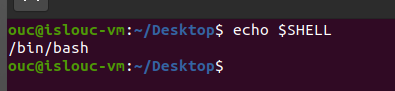
\includegraphics[width=1\textwidth]{1.png}
\end{figure}
\begin{figure}[H]
    \centering
    练习2:
    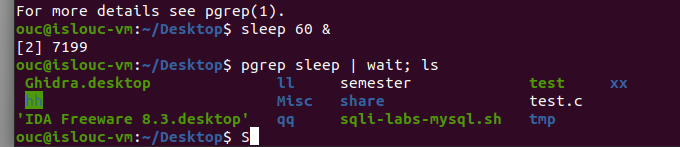
\includegraphics[width=1\textwidth]{2.png}
\end{figure}
\begin{figure}[H]
    \centering
    练习3:
    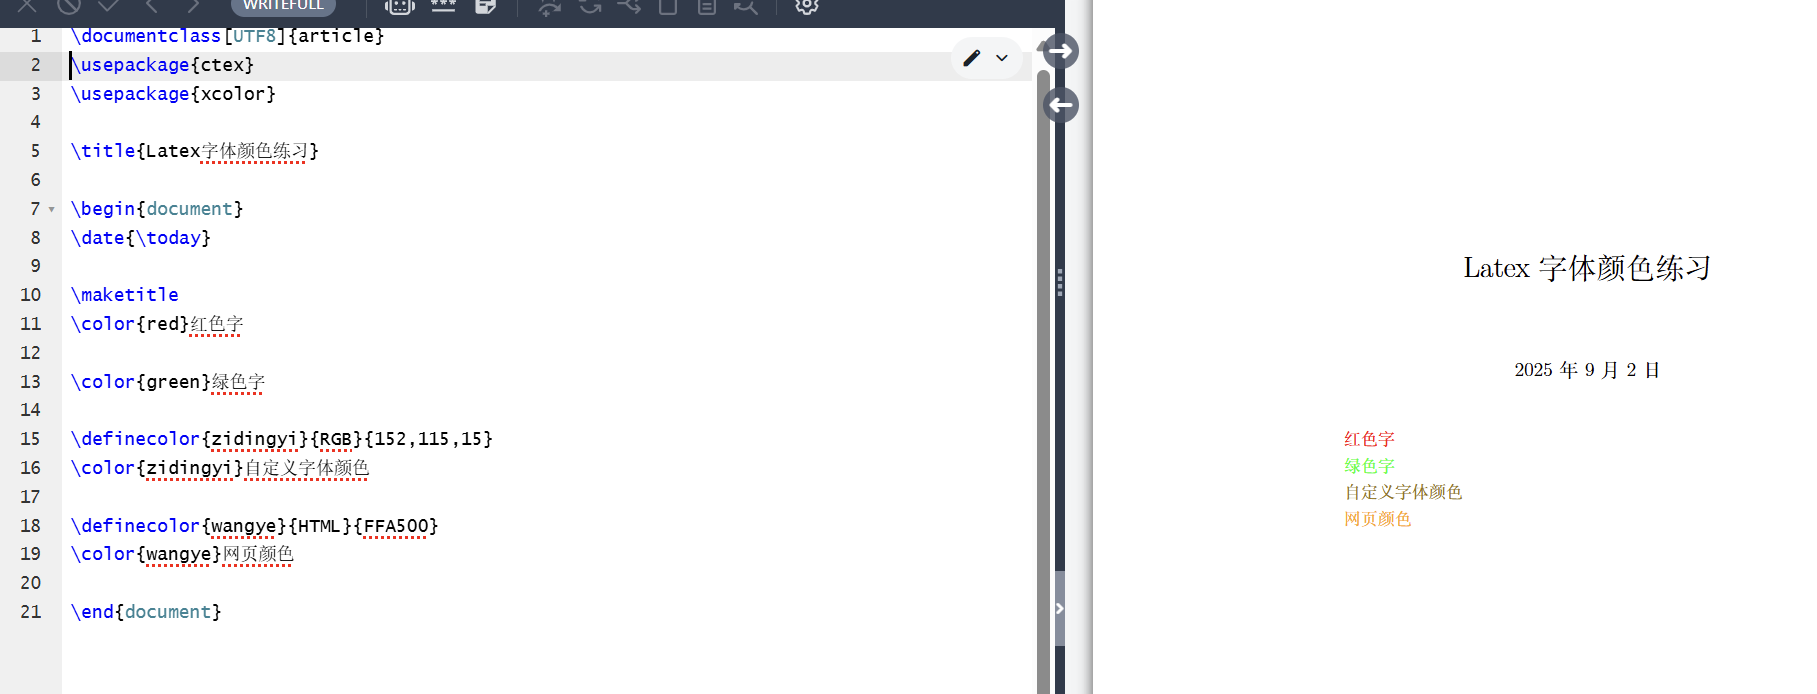
\includegraphics[width=1\textwidth]{3.png}
\end{figure}
\begin{figure}[H]
    \centering
    练习4:
    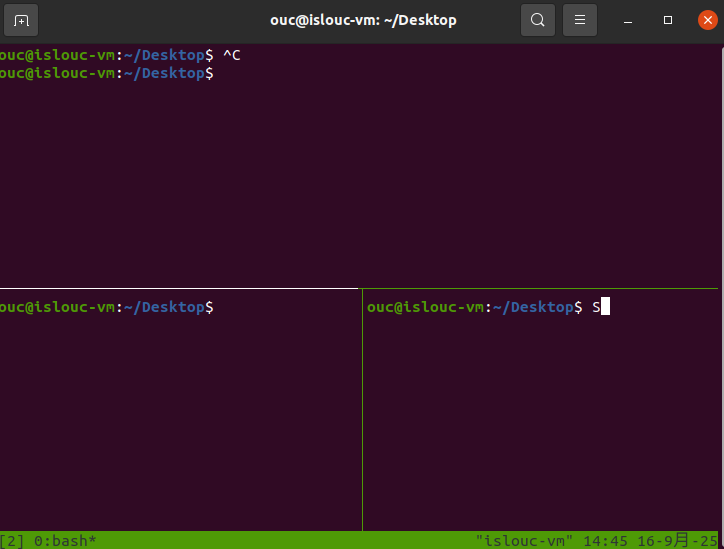
\includegraphics[width=1\textwidth]{4.png}
\end{figure}
\begin{figure}[H]
    \centering
    练习5:
    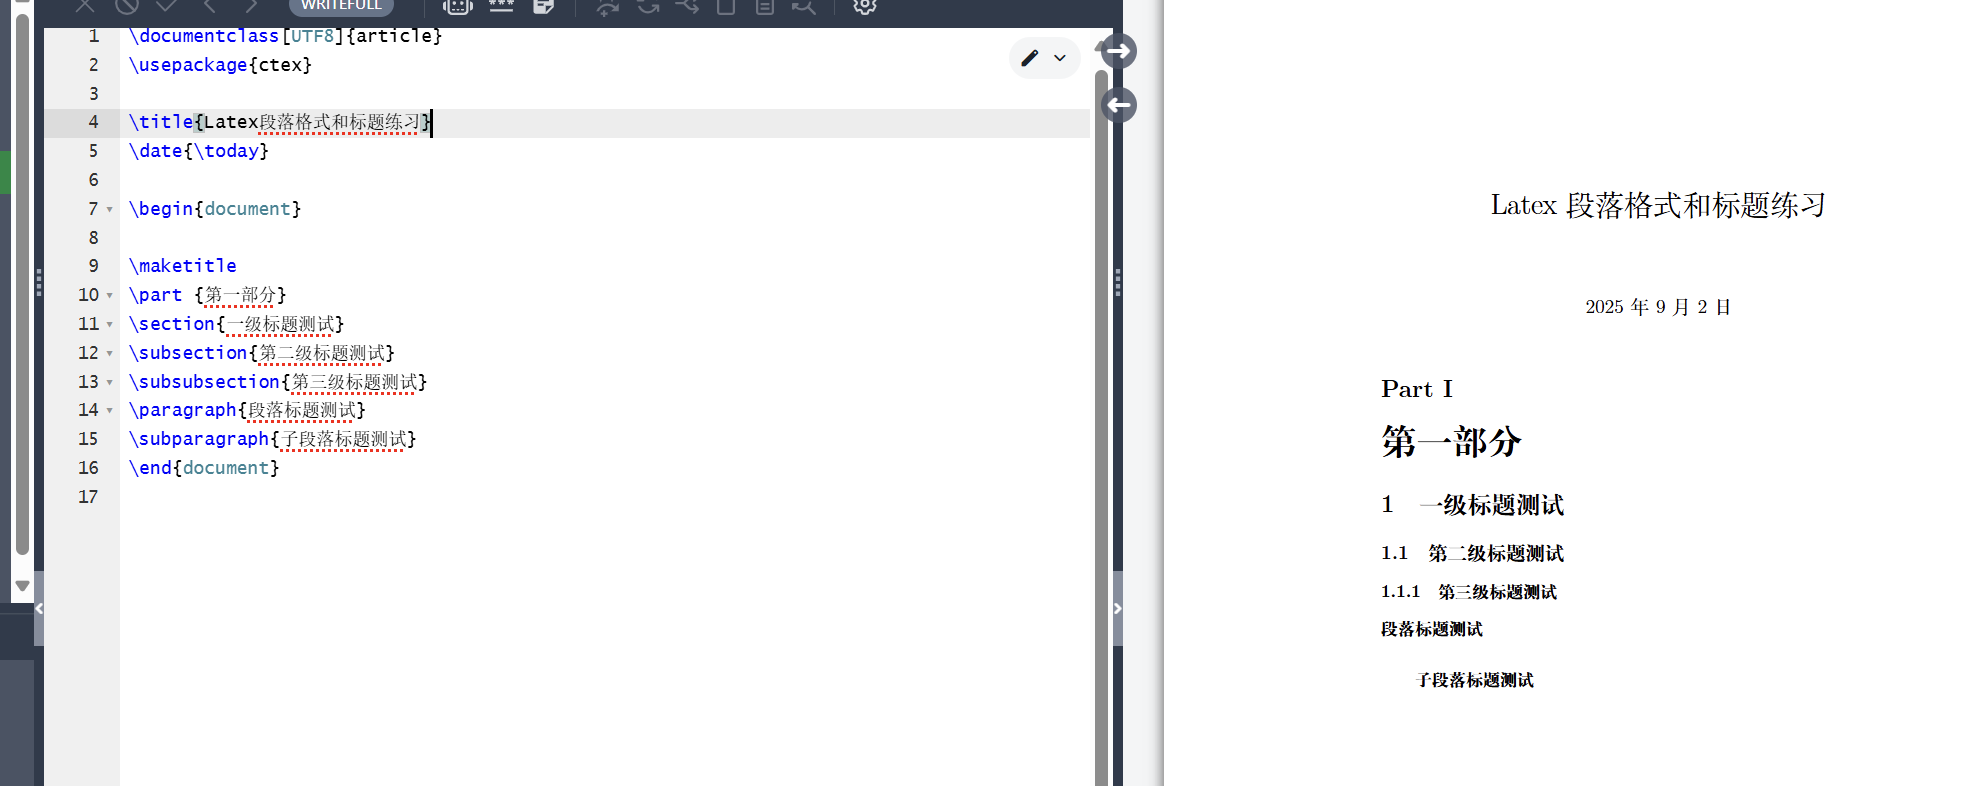
\includegraphics[width=1\textwidth]{5.png}
\end{figure}
\begin{figure}[H]
    \centering
    练习6:
    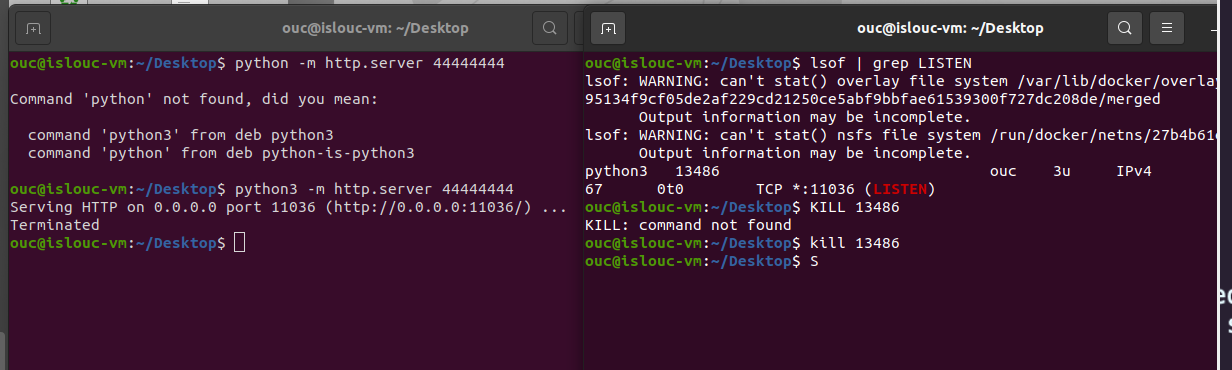
\includegraphics[width=1\textwidth]{6.png}
\end{figure}
\begin{figure}[H]
    \centering
    练习7:
    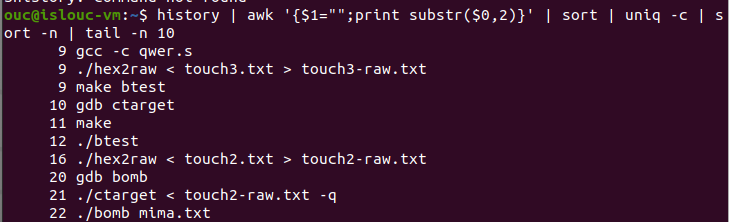
\includegraphics[width=1\textwidth]{7.png}
\end{figure}
\begin{figure}[H]
    \centering
    练习8:
    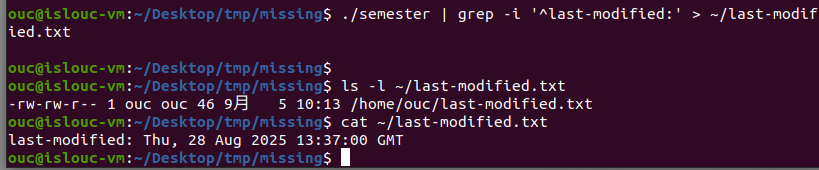
\includegraphics[width=1\textwidth]{8.png} 
\end{figure}
\begin{figure}[H]
    \centering
    练习9:
    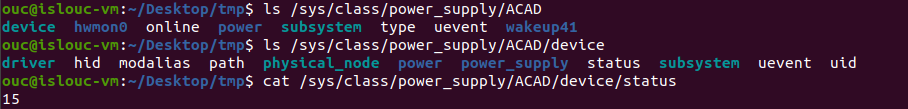
\includegraphics[width=1\textwidth]{9.png}
\end{figure}
\begin{figure}[H]
    \centering
    练习10:
    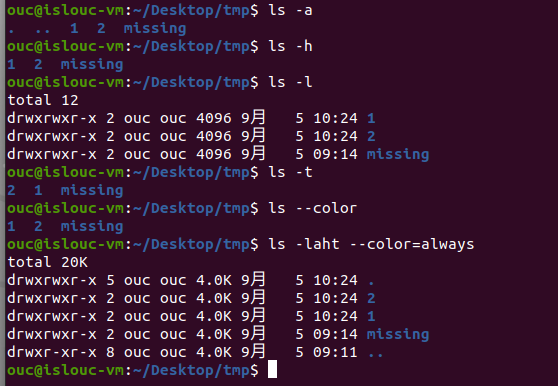
\includegraphics[width=1\textwidth]{10.png}
\end{figure}
\begin{figure}[H]
    \centering
    练习11:
    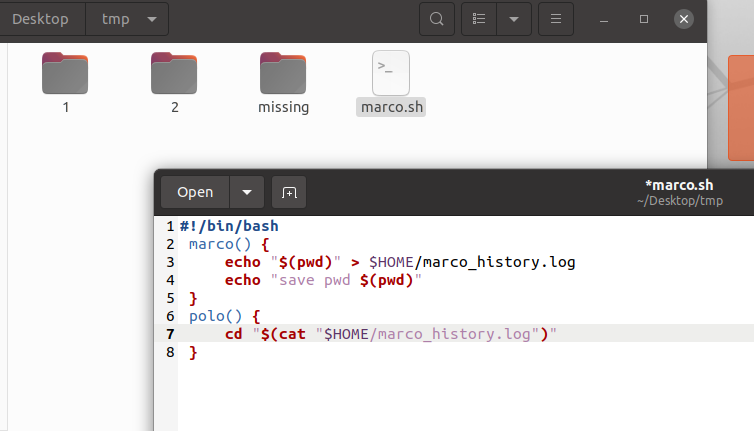
\includegraphics[width=1\textwidth]{11.png}
\end{figure}
\begin{figure}[H]
    \centering
    练习12:
    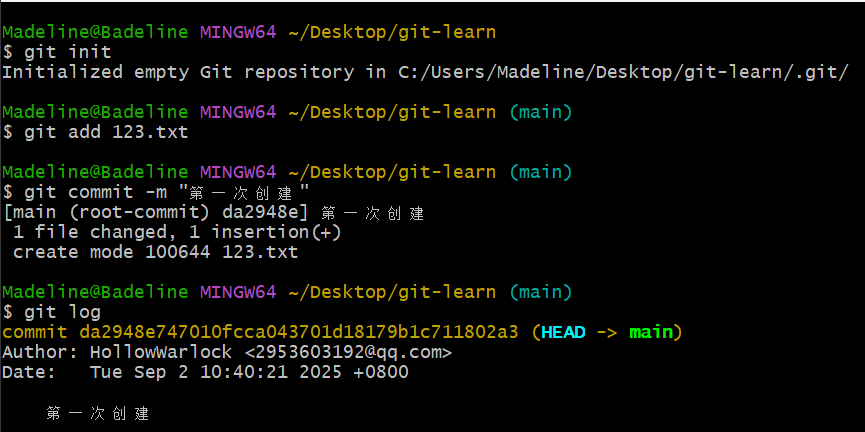
\includegraphics[width=1\textwidth]{12.png}
\end{figure}
\begin{figure}[H]
    \centering
    练习13:
    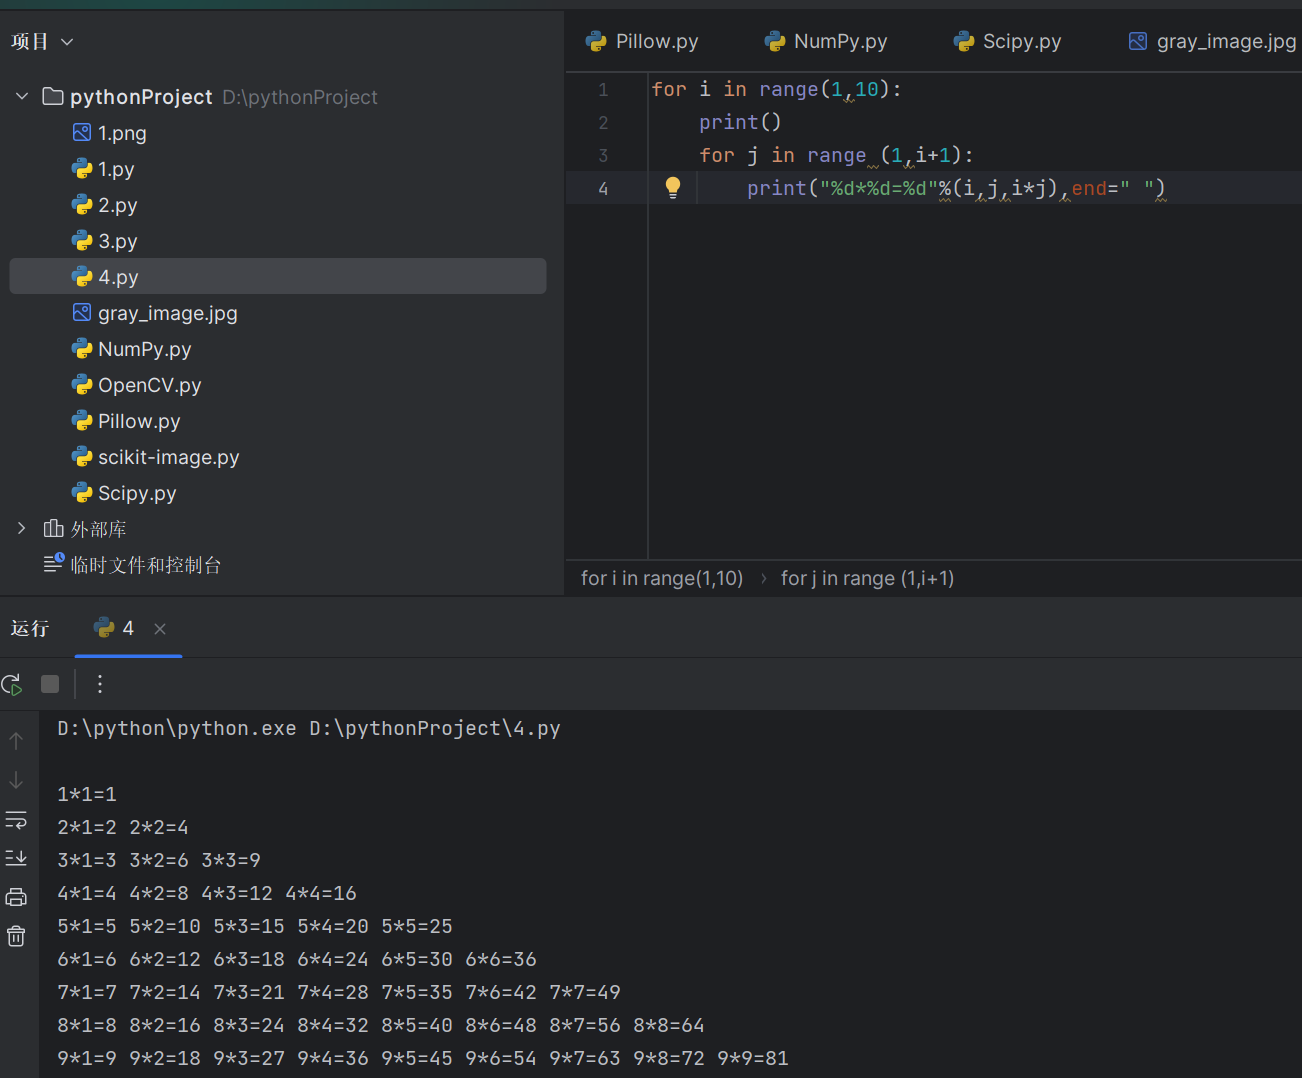
\includegraphics[width=1\textwidth]{13.png}
    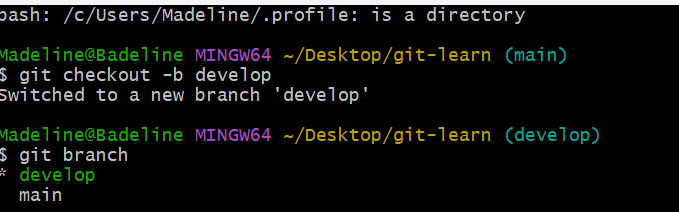
\includegraphics[width=1\textwidth]{14.png}
    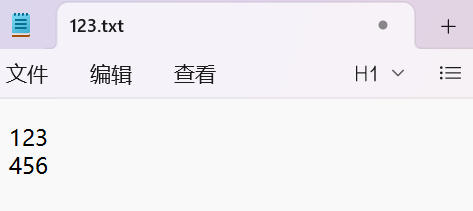
\includegraphics[width=1\textwidth]{15.png}
    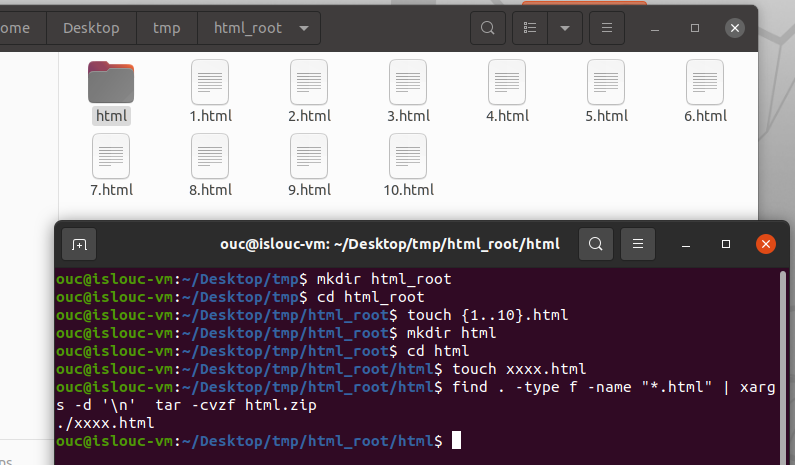
\includegraphics[width=1\textwidth]{16.png}
    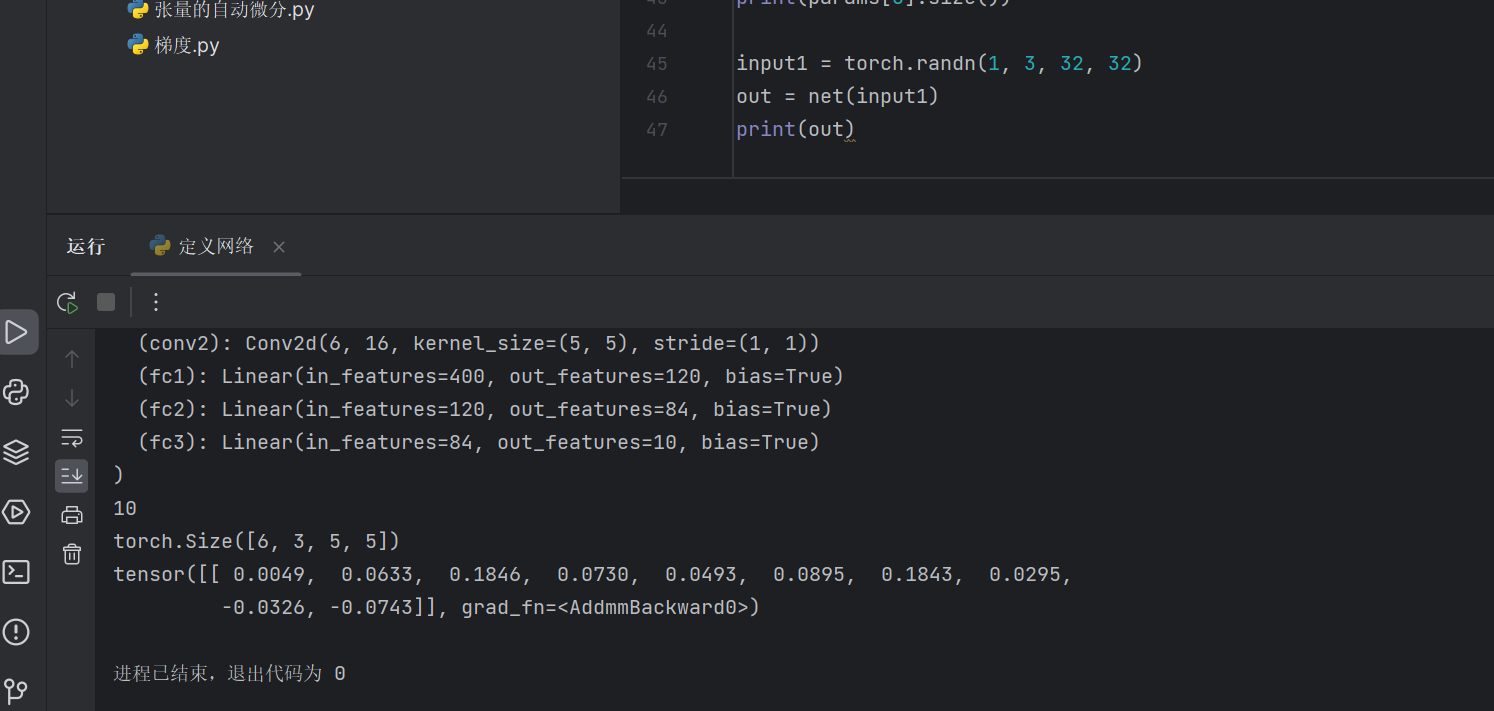
\includegraphics[width=1\textwidth]{17.png}
\end{figure}
\begin{figure}[H]
    \centering
    练习14:
    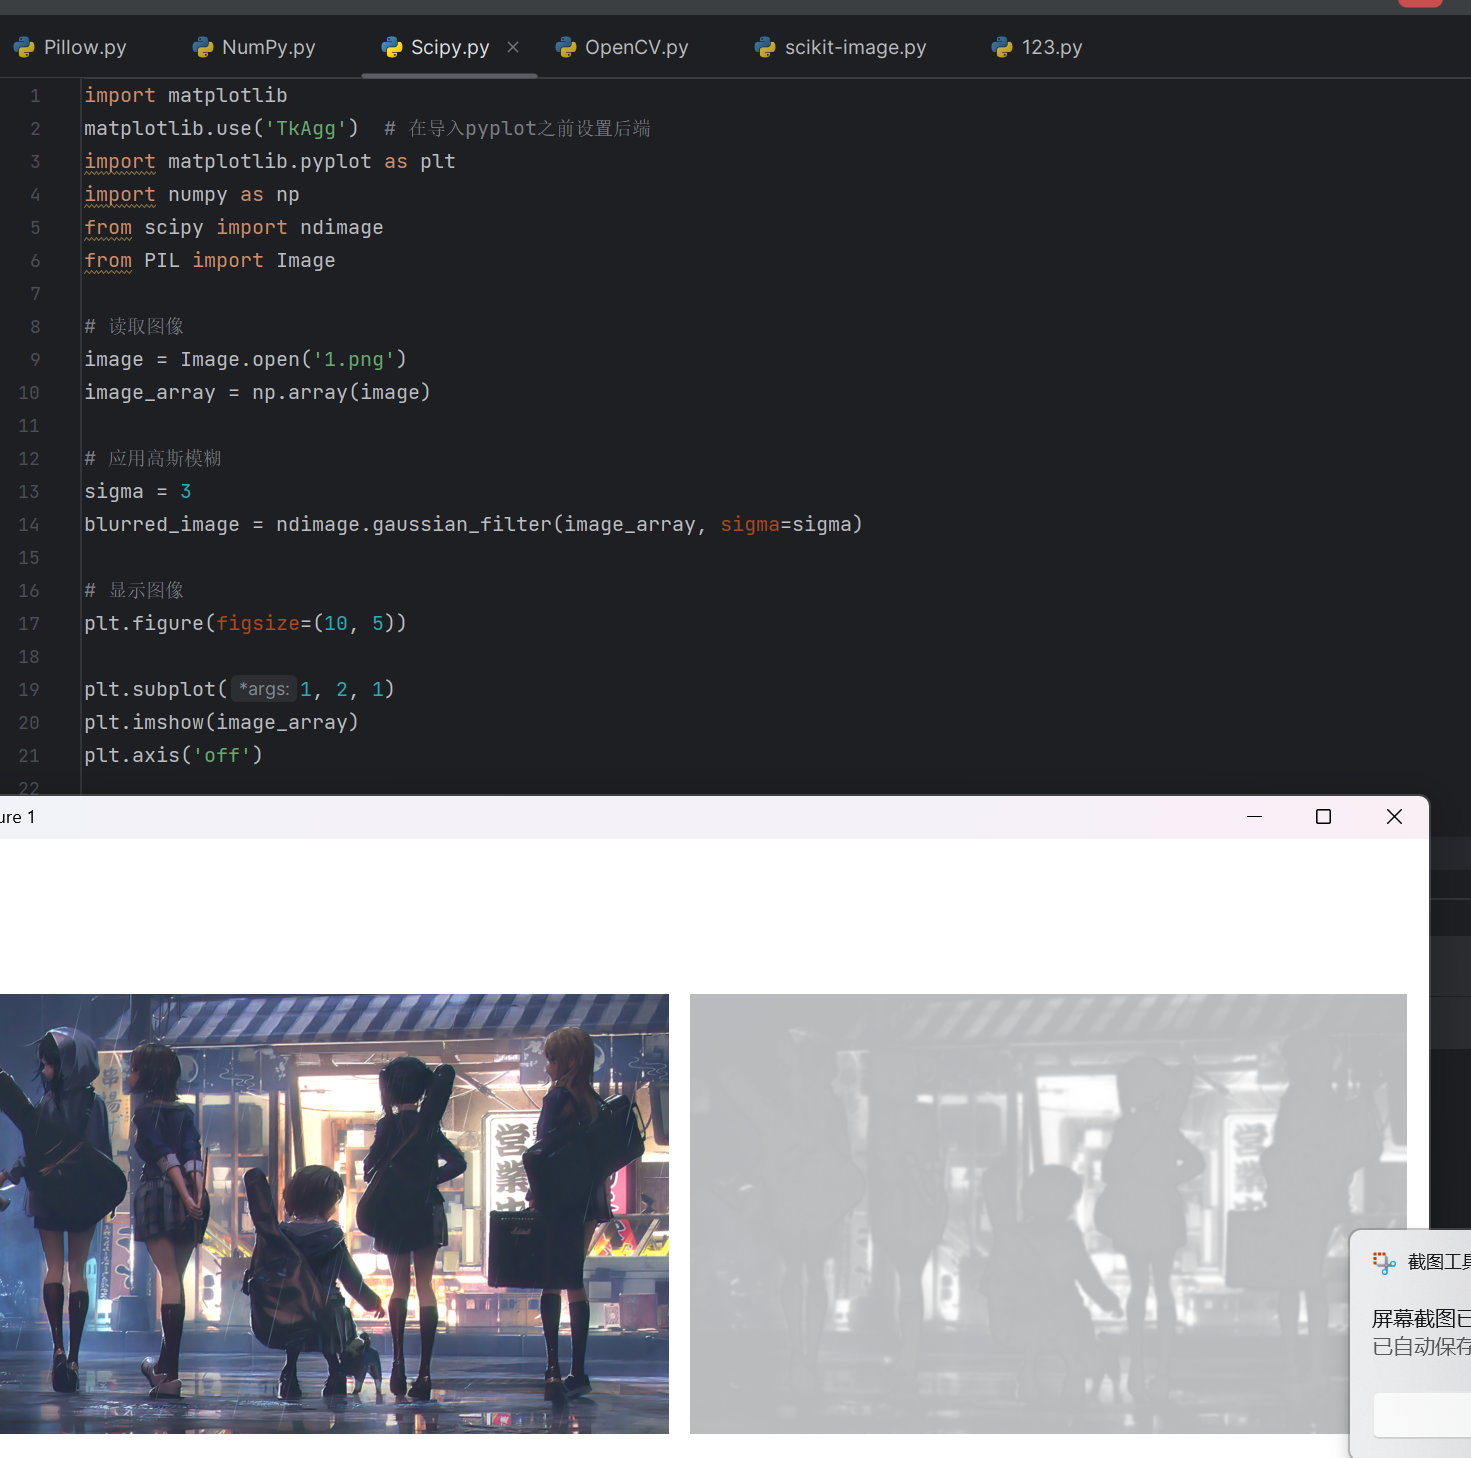
\includegraphics[width=1\textwidth]{18.png}
    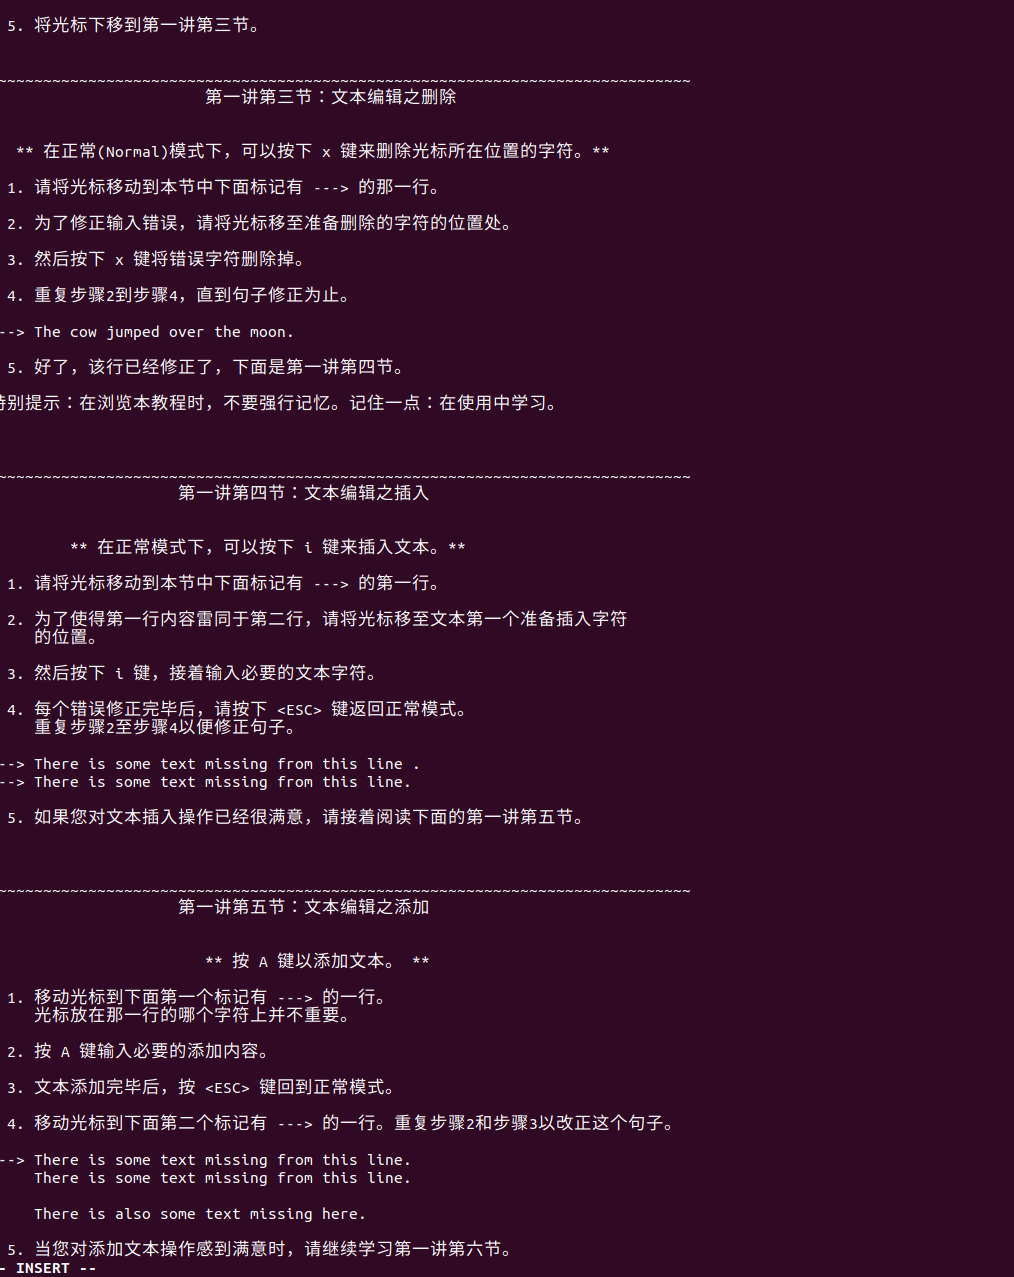
\includegraphics[width=1\textwidth]{19.png}
    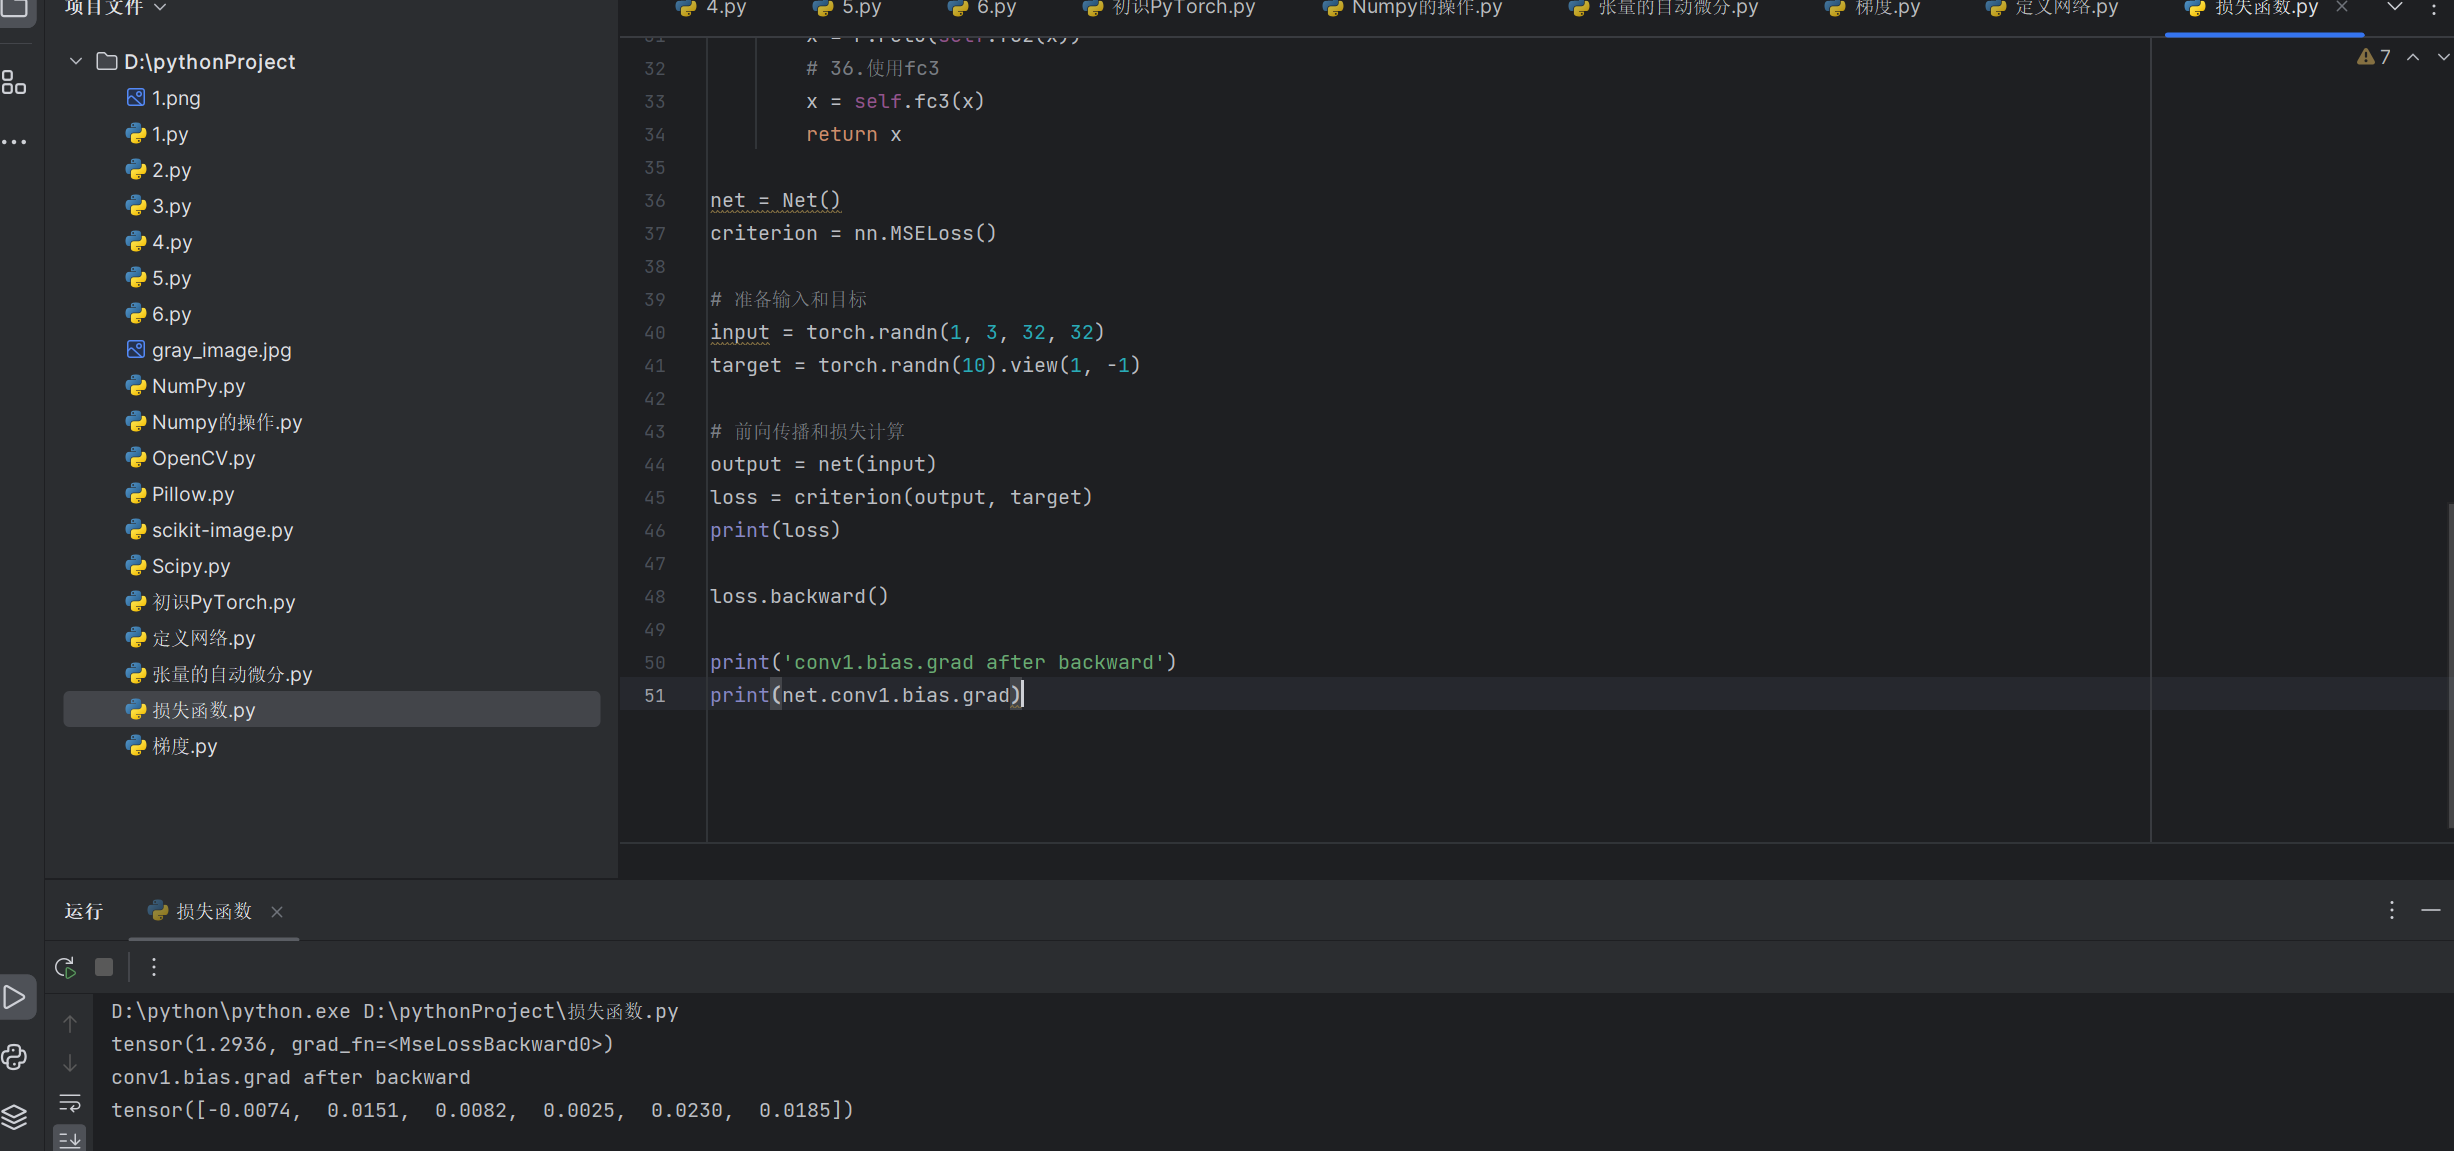
\includegraphics[width=1\textwidth]{20.png}
\end{figure}
\begin{figure}[H]
    \centering
    练习15:
    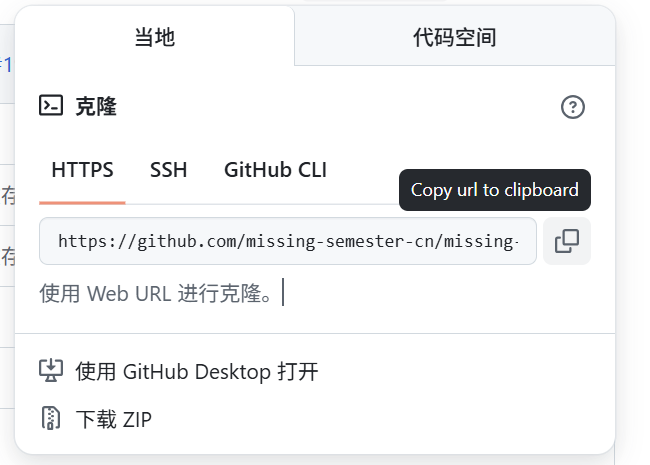
\includegraphics[width=1\textwidth]{21.png}
    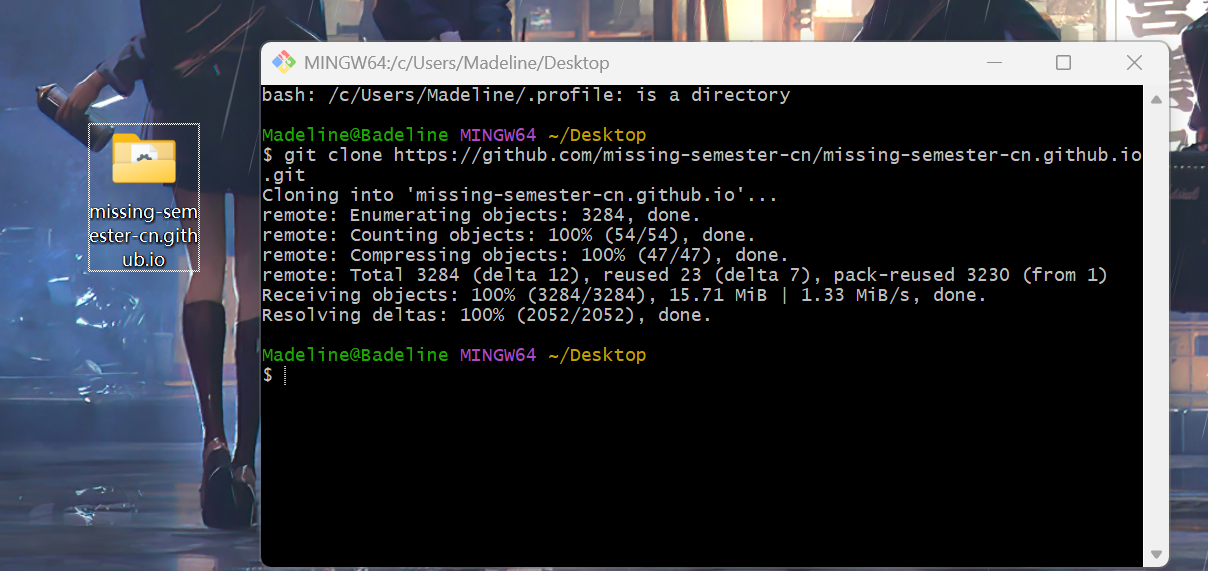
\includegraphics[width=1\textwidth]{22.png}
\end{figure}
\begin{figure}[H]
    \centering
    练习16:
    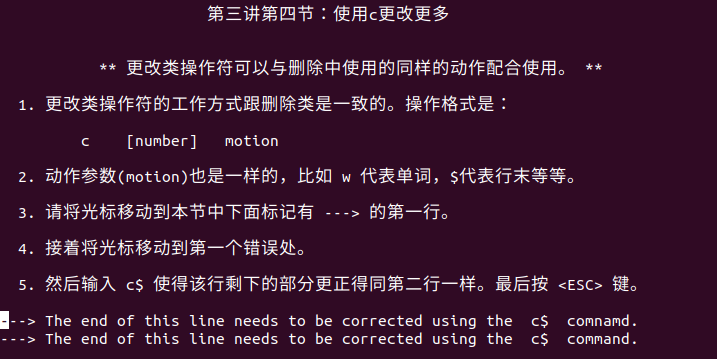
\includegraphics[width=1\textwidth]{23.png}
    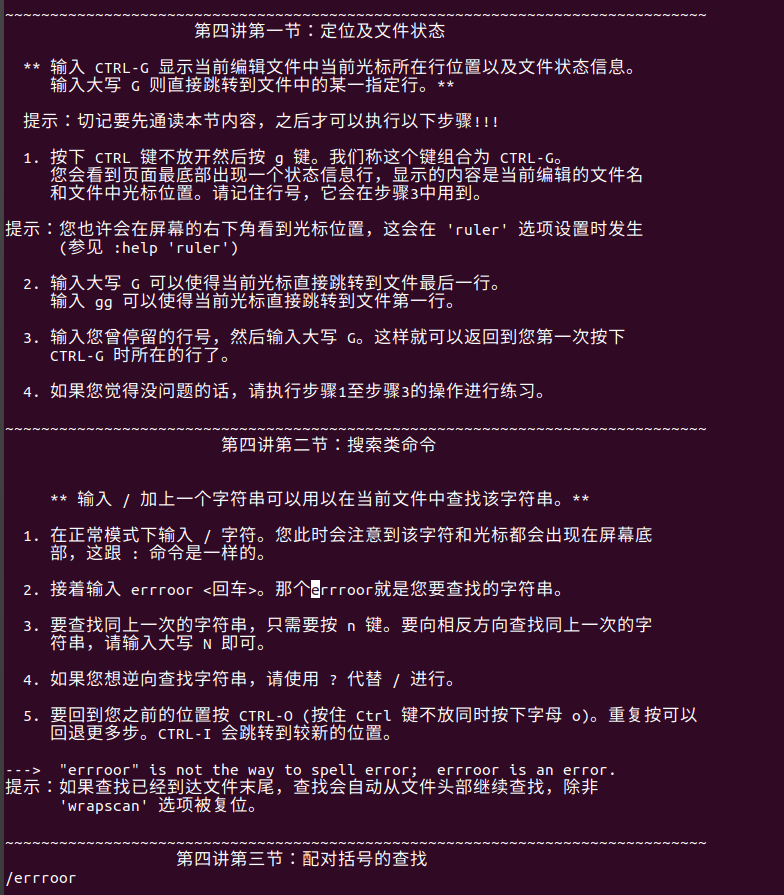
\includegraphics[width=1\textwidth]{24.png}
    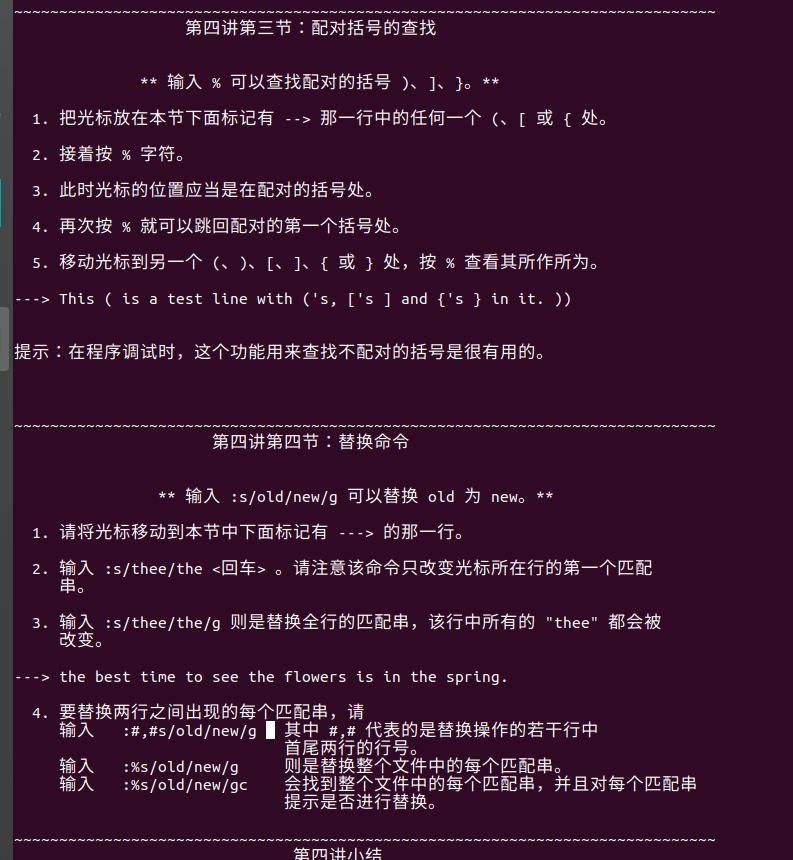
\includegraphics[width=1\textwidth]{25.png}
\end{figure}
\begin{figure}[H]
    \centering
    练习17:
    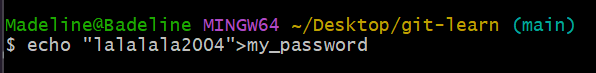
\includegraphics[width=1\textwidth]{26.png}
    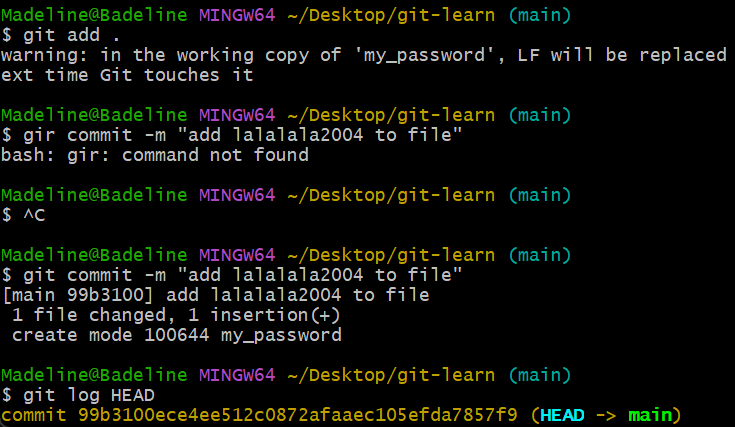
\includegraphics[width=1\textwidth]{27.png}
    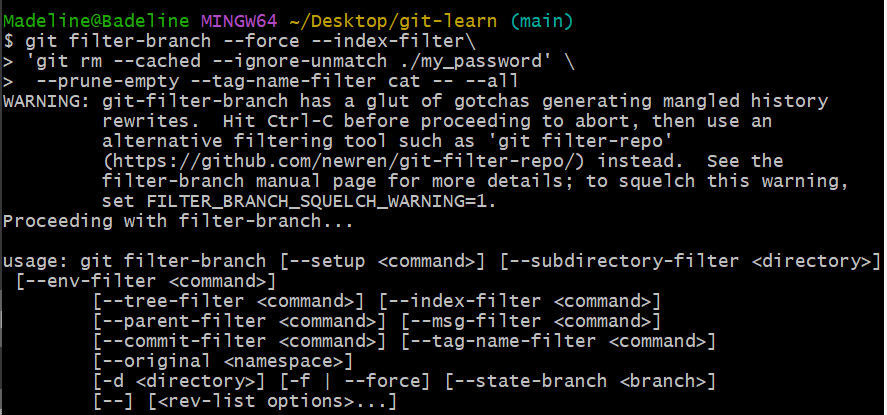
\includegraphics[width=1\textwidth]{28.png}
\end{figure}
\begin{figure}[H]
    \centering
    练习18:
    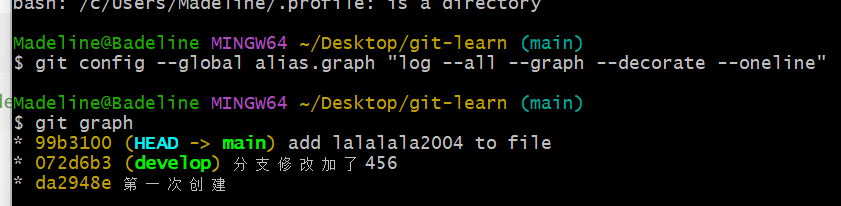
\includegraphics[width=1\textwidth]{29.png}
\end{figure}
\begin{figure}[H]
    \centering
    练习19:
    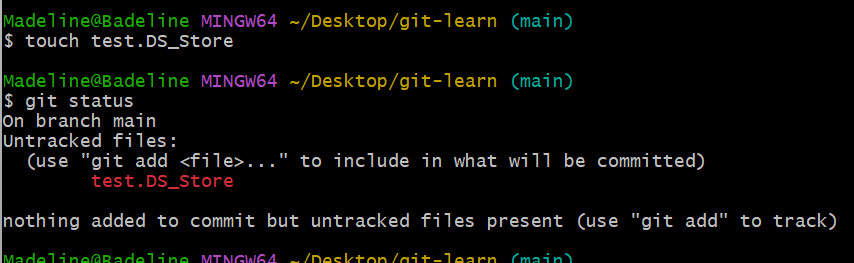
\includegraphics[width=1\textwidth]{30.png}
\end{figure}
\begin{figure}[H]
    \centering
    练习20:
    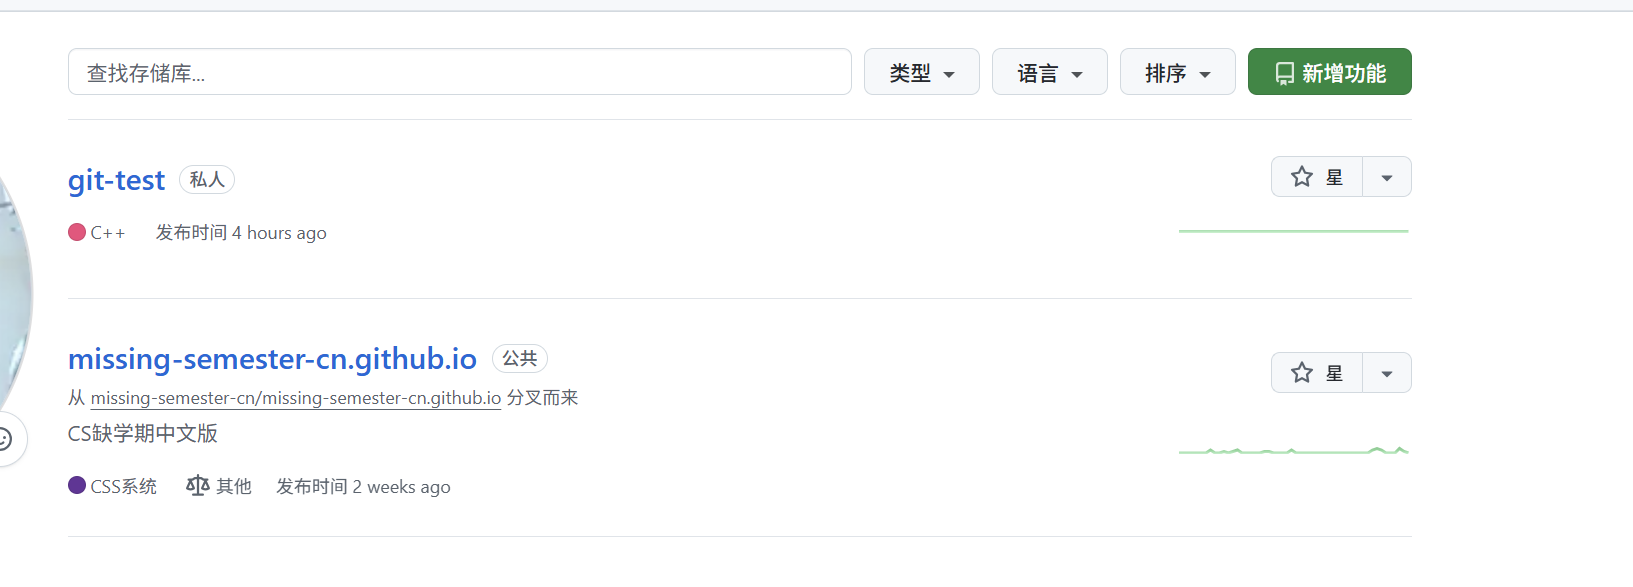
\includegraphics[width=1\textwidth]{31.png}
\end{figure}

% 第三段:结尾


\section{体会与收获}
通过本次实验我基本掌握了Latex的用法,主要是了解到了Latex在论文和文章排版中的作用和定位。我觉得刚起步使用Latex是一件复杂且不直观的事情,但是熟悉语法后可以省下很多排版上的麻烦,并且可以统一很多的格式,尤其是论文方面的排版,让文献都有一个较为统一的格式是很方便的事情。
在写Latex实验过程中,我遇到了一些排版问题,图片的位置总是出错。最后是用了float宏包的H参数解决的问题。

其次就是我在本次实验中着重学会了使用Git,Git是一个非常便捷的工具,尤其是衍生出的Github平台,让代码之间的交流变得简单快捷,我只是简单地使用Git创建了一些文档,但很明显在版本的更迭开发中Git有着更大的作用。
我通过Github接触到了程序员之间的交流,感到兴奋和开源的伟大。
在使用Github中我遇到了上不去网站的情况,最后使用了Watt Toolkit工具才流畅进入。



github地址:https://github.com/HollowWarlock/ouc-xitonggongjukaifajichu.git

\end{document}